\chapter{Complex Algebra and Phasor Notation}
\label{chap:complexAlgebra}
In the last chapter, I introduced the concept of \textit{impedance}, which is a complex quantity that relates the voltage across a circuit element to the current through that element. From this point on in the course, impedance will supercede resistance in our calculations of circuit behavior. For that reason, and because impedance calculations require an understanding of complex algebra, this chapter will just focus on representations of complex numbers and on rules for adding, subtracting, multiplying, and dividing them. Think of this chapter as a complex algebra-focused interlude. 

\section{Representations of Complex Numbers}
A complex number is comprised of two parts: its real part, and its imaginary part. One way to represent complex numbers is by expressing their real and imaginary parts separately. Think of this as a vector in the two-dimensional complex plane. This is called the \textbf{Cartesian} form for a complex number, because it easily maps to a Cartesian coordinate system with real numbers along the horizontal axis and imaginary numbers along the vertical axis as shown in Figure \ref{cartesianZ}. In this figure, the real and imaginary parts of Z provide the horizontal and vertical coordinates of Z in the complex plane, respectively. The Cartesian form for a generic complex number $Z$ is expressed as follows:
$$
\textbf{Cartesian form:}\textnormal{                         }Z=\underbrace{a}_{\textnormal{real part}} + \underbrace{j\cdot b}_{\textnormal{imaginary part}}
$$
\begin{figure}[h!]
\centering
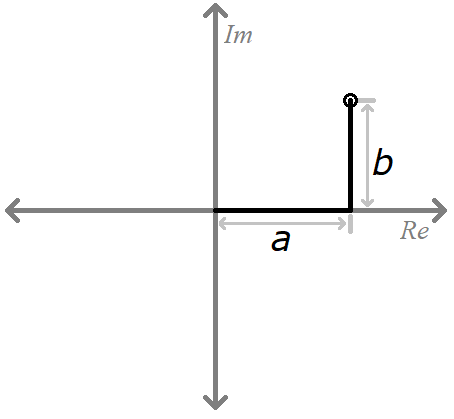
\includegraphics[width=5cm]{figures/ZCartesian.png}
\caption{The complex number Z mapped onto the complex plane using Cartesian coordinates.}
\label{cartesianZ}
\end{figure}
\par
Another way to represent complex numbers is by specifying the magnitude of the vector and a phase angle. This is called the \textbf{polar} form for a complex number, because it easily maps to a polar coordinate system in the complex plane, as shown in Figure \ref{polarZ}. The plane in this figure is still real on the horizontal axis and imaginary along the vertical axis. Now, however, the complex number is plotted by rotating counter-clockwise from the positive real axis to the specified phase angle and then plotting a line out from the origin by the specified magnitude. In other words, the magnitude and angle of Z indicate how far Z is from the origin and what angle Z sweeps out with respect to the positive real axis, respectively. 
\begin{figure}[h!]
\centering
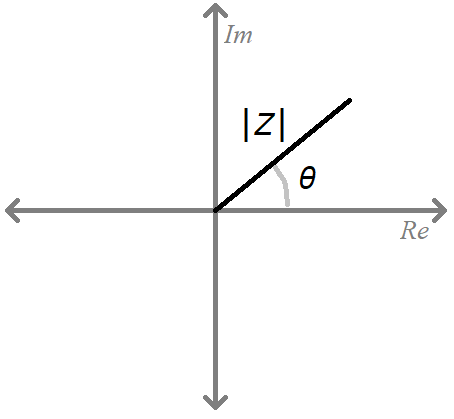
\includegraphics[width=5cm]{figures/ZPolar.png}
\caption{The complex number Z mapped onto the complex plane using Polar coordinates.}
\label{polarZ}
\end{figure}
We will often write the polar form in an abbreviated way known as the \textbf{phasor} representation of the number. The polar and phasor forms for a generic complex number are given below: 
$$
\textbf{Polar form:}\textnormal{                 } Z = |Z|e^{j\theta}
$$
$$
\textbf{Phasor form:}\textnormal{                 } Z = |Z|\angle\theta
$$
\par
As we will see in the next section, it is nice to have more than one way to represent complex numbers because some arithmetic operations are easier with one form than the other. If we ever need to convert a complex number from Cartesian form to polar form or vice versa, we can do so using the following rules:
$$
\textbf{Converting Cartesian to polar form: }a + j\cdot b = \sqrt{a^2 + b^2}e^{j(\arctan(b/a))}
$$
$$
\textbf{Converting polar to Cartesian form}\footnote{Remember Euler's formula: $e^{j\theta} = cos\theta + j sin\theta$}\textbf{: }|Z|e^{j\theta} = |Z|\cos(\theta) + j\cdot |Z|\sin(\theta)
$$


\section{Adding, Subtracting, Multiplying, and Dividing Complex Numbers}
When we add or subtract complex numbers, it is easiest to do so using their Cartesian form, because the real parts and the imaginary parts need to be added or subtracted separately from each other. If we need to add complex numbers that are in phasor or polar form, it's best to convert them to Cartesian form first. Here are the rules for addition and subtraction of complex numbers, using two generic complex numbers $Y=a+j\cdot b$ and $Z=c+j\cdot d$:
$$
(Y+Z) = (a+c) + j\cdot(b+d)
$$
$$
(Y-Z) = (a-c) + j\cdot(b-d)
$$
\par
When we multiply or divide complex numbers, it is easiest to do so using their polar or phasor form, because this reduces the amount of tedious arithmetic we must do to obtain the result. If we need to multiply two complex numbers, we could do so using Cartesian form, but it's easiest in polar form. And, when we need to divide two complex numbers, it is best to convert both to polar or phasor form. Here are the rules for multiplication and division of complex numbers using two generic complex numbers $Y = |Y|\angle\theta$ and $Z = |Z|\angle\phi$:
$$
(Y\cdot Z) = (|Y|\cdot|Z|)\mathlarger{\angle}(\theta+\phi)
$$
$$
\left(\frac{Y}{Z}\right) = \left(\frac{|Y|}{|Z|}\right)\mathlarger{\angle}(\theta-\phi)
$$
We can also multiply two complex numbers in Cartesian form if necessary (using the F.O.I.L. method), but remember that $j\cdot j=-1$. Using two generic complex numbers $Y=a+j\cdot b$ and $Z=c+j\cdot d$:
$$
(Y\cdot Z) = (a+j\cdot b)\cdot(c+j\cdot d) = (a\cdot c) + j\cdot (b\cdot c) + j\cdot(a\cdot d) + \cancelto{-1}{j^2}\cdot (b\cdot d) 
$$
$$
= [(a\cdot c) - (b\cdot d)] + j\cdot[(b\cdot c) + (a\cdot d)]
$$
\section{Shortcuts with $j$}
Like many things in life, the main way you will get better at complex algebra is through practice using it. However the tricks in this section will save you lots of time if you remember them because they are really useful in the context of circuits, and they seem to come up often.
\par
You may sometimes find these angle-to-imaginary-number relationships useful when you are needing to convert a complex number from Cartesian to phasor form or vice versa:
$$
\angle{90^{\circ}} = \angle\left(\frac{\pi}{2}\right) = j
$$
$$
\angle{-90^{\circ}} = \angle{-\left(\frac{\pi}{2}\right)} = -j
$$
$j$ is tricky, and sometimes it shows up where it shouldn't. The following equations give you easy ways to push $j$ around.
$$
j^2 = -1
$$
$$
\frac{1}{j} = -j
$$
\section{Back to Circuits: Complex Impedance}
Remember that Ohm's law defines \textit{resistance} as the ratio of voltage across the resitor to the current flowing through that resistor. If we extend Ohm's law into the domain of complex numbers, a more general version of Ohm's law emerges:
$$
V = i \cdot Z
$$
This is not too impressive on the surface, but now in the place of a fully-\textit{real} resistance, $R$, we have a complex-valued \textbf{impedance}, $Z$. Impedance can be broken into two parts:
$$
Z = \underbrace{R}_{Resistance} + \textrm{  } j \cdot \underbrace{X}_{\mathclap{Reactance}}
$$
\par
From the above definition, we see that the resistance is the real part of impedance. We call the complex part of impedance reactance. This means that the resistance we have studied so far is a special case of the larger concept of impedance. In Chapter \ref{chap:capInductorProperties}, we derived the impedance for capacitors and inductors under sinusoidal driving conditions. Capacitor and inductor impedances are purely \textit{reactive}. Using the conversion techniques of this chapter, those impedances are represented in Cartesian and phasor form as follows:
$$
Z_C = \frac{1}{j\omega C} = \frac{-j}{\omega C} = \left(\frac{1}{\omega C}\right)\mathlarger{\mathlarger{\angle}}-\left(\frac{\pi}{2}\right)
$$
$$
Z_L = j\omega L = \omega L\mathlarger{\mathlarger{\angle}}\left(\frac{\pi}{2}\right)
$$
Now that we've covered the rules for manipulating complex numbers, we can use these expressions for impedance along with resistance to analyze AC circuit behavior.

\section{Recap: Representing and Manipulating Complex Numbers}
Complex numbers may seem obscure; anything we un-ironically refer to as ``imaginary'' really does warrant some careful explanation. However, the representations of and rules for manipulating complex numbers presented in this chapter will be very useful as we proceed with the rest of the course. This recap might come in handy as a reference.
\begin{description}
\item[Cartesian form:]
$$
Z=\underbrace{a}_{\textnormal{real part}} + \underbrace{j\cdot b}_{\textnormal{imaginary part}}
$$
\item[Polar form:]
$$
Z = |Z|e^{j\theta}
$$
\item[Phasor form:]
$$
Z = |Z|\angle\theta
$$
\item[Converting Cartesian to Polar and Phasor Form:]
$$
a + j\cdot b = \sqrt{a^2 + b^2}e^{j(\arctan(b/a))} = \sqrt{a^2 + b^2}\angle(\arctan(b/a))
$$
\item[Converting polar to Cartesian form:]
$$
|Z|e^{j\theta} = |Z|\cos(\theta) + j\cdot |Z|\sin(\theta)
$$
\item[Addition and Subtraction of Complex Numbers:] This is done in Cartesian form. Using two generic complex numbers $Y=a+j\cdot b$ and $Z=c+j\cdot d$:
$$
(Y+Z) = (a+c) + j\cdot(b+d)
$$
$$
(Y-Z) = (a-c) + j\cdot(b-d)
$$
\item[Multiplication and Division of Complex Numbers:] This is done in polar or phasor form. Using two generic complex numbers $Y = |Y|\angle\theta$ and $Z = |Z|\angle\phi$:
$$
(Y\cdot Z) = (|Y|\cdot|Z|)\mathlarger{\angle}(\theta+\phi)
$$
$$
\left(\frac{Y}{Z}\right) = \left(\frac{|Y|}{|Z|}\right)\mathlarger{\angle}(\theta-\phi)
$$
We can also multiply two complex numbers in Cartesian form. Using two generic complex numbers $Y=a+j\cdot b$ and $Z=c+j\cdot d$:
$$
(Y\cdot Z) = [(a\cdot c) - (b\cdot d)] + j\cdot[(b\cdot c) + (a\cdot d)]
$$
\item[Additional representations for $j$:] 
$$
\angle90^{\circ} = j
$$
$$
\angle-90^{\circ} = -j
$$
$$
j^2 = -1
$$
$$
\frac{1}{j} = -j
$$
\item[Impedance:] The complex ratio of voltage across to current flowing through a passive circuit element. Resistance is the \textit{real} part of impedance:
$$
Z = \underbrace{R}_{Resistance} + \textrm{  } j \cdot \underbrace{X}_{\mathclap{Reactance}}
$$



\end{description}